\documentclass[10pt]{article}
% Math Packages
\usepackage{amsmath, mathtools}
\usepackage{amssymb}
\usepackage{amsthm}
\usepackage{amsfonts}
\usepackage{bbm}
\usepackage{breqn}
\usepackage[margin=1in]{geometry}
\usepackage{graphicx}
\usepackage{tikz}
\usetikzlibrary{arrows.meta}
\usetikzlibrary{calc}
\usepackage{forest}
\usepackage{tikz-qtree}
\graphicspath{ {./images/} }
\usepackage{hyperref}
\usepackage[capitalize]{cleveref}
\usepackage[shortlabels]{enumitem}
\usetikzlibrary{arrows,matrix,positioning}
\usepackage{multicol}

% for the pipe symbol
\usepackage[T1]{fontenc}

% Citing theorems by name. (source: https://tex.stackexchange.com/questions/109843/cleveref-and-named-theorems)
\makeatletter
\newcommand{\ncref}[1]{\cref{#1}\mynameref{#1}{\csname r@#1\endcsname}}

\def\mynameref#1#2{%
  \begingroup
  \edef\@mytxt{#2}%
  \edef\@mytst{\expandafter\@thirdoffive\@mytxt}%
  \ifx\@mytst\empty\else
  \space(\nameref{#1})\fi
  \endgroup
}
\makeatother

% Colorful Notes
\usepackage{color} \definecolor{Red}{rgb}{1,0,0} \definecolor{Blue}{rgb}{0,0,1}
\definecolor{Purple}{rgb}{.5,0,.5} \def\red{\color{Red}} \def\blue{\color{Blue}}
\def\gray{\color{gray}} \def\purple{\color{Purple}}
\newcommand{\rnote}[1]{{\red [#1]}} % \rnote{foo} gives '[foo]' in red
\newcommand{\pnote}[1]{{\purple [#1]}} % \pnote{foo} gives '[foo]' in purple
\newcommand{\bnote}[1]{{\blue #1}} % \bnote{foo} gives 'foo' in blue
\newcommand{\gnote}[1]{{\gray #1}} % \gnote{foo} gives 'foo' in gray
\newcommand{\Max}[1]{{\purple [#1]}} % \bnote{foo} then 'foo' is blue


% Claim numbering (the counter restarts after each proof environment)
\newcounter{claimcount}
\setcounter{claimcount}{0}
\newenvironment{claim}{\refstepcounter{claimcount}\par\addvspace{\medskipamount}\noindent\textbf{Claim \arabic{claimcount}:}}{}
\usepackage{etoolbox}
\AtBeginEnvironment{proof}{\setcounter{claimcount}{0}}
\newenvironment{claimproof}{\par\addvspace{\medskipamount}\noindent\textit{Proof of Claim  \arabic{claimcount}.}}{\hfill\ensuremath{\qedsymbol} \tiny{Claim}

  \medskip}
% Add claim support to cleverref
\crefname{claimcount}{Claim}{Claims}


% Math Environments
\newtheorem{theorem}{Theorem}
\newtheorem{assumption}[theorem]{Assumption}
\newtheorem{lemma}[theorem]{Lemma}
\newtheorem{proposition}[theorem]{Proposition}
\newtheorem{corollary}[theorem]{Corollary}
\newtheorem{question}[theorem]{Question}
\theoremstyle{definition}
\newtheorem{definition}[theorem]{Definition}
\newtheorem{remark}[theorem]{Remark}
\newtheorem{example}[theorem]{Example}
\newtheorem{notation}[theorem]{Notation}
\newtheorem{problem}[theorem]{Problem}

% Matrices and Column Vectors. 
\usepackage{stackengine}
\setstackgap{L}{1.0\normalbaselineskip}
\usepackage{tabstackengine}
\setstackEOL{;}% row separator
\setstackTAB{,}% column separator
\setstacktabbedgap{1ex}% inter-column gap
\setstackgap{L}{1.5\normalbaselineskip}% inter-row baselineskip
\let\nmatrix\bracketMatrixstack  %Usage: \nmatrix{1,2,3\4,5,6}
\newcommand\cv[1]{\setstackEOL{,}\bracketMatrixstack{#1}} %usage: \cv{1,2,3}

% Custom Math Coqmmands
\newcommand{\vt}{\vskip 5mm} % vertical space
\newcommand{\fl}{\noindent\textbf} % first line
\newcommand{\Fl}{\vt\noindent\textbf} % first line with space above
\newcommand{\norm}[1]{\left\lVert#1\right\rVert} % norm
\newcommand{\pnorm}[1]{\left\lVert#1\right\rVert_p} % p-norm
\newcommand{\qnorm}[1]{\left\lVert#1\right\rVert_q} % q-norm
\newcommand{\1}[1]{\textbf{1}_{\left[#1\right]}} % indicator function 
\def\limn{\lim_{n\to\infty}} % shortcut for lim as n-> infinity
\def\sumn{\sum_{n=1}^{\infty}} % shortcut for sum from n=1 to infinity
\def\sumkn{\sum_{k=1}^{n}} % shortcut for sum from k=1 to n
\def\sumin{\sum_{i=1}^{n}} % shortcut for sum from i=1 to n
\def\SAs{\sigma\text{-algebras}} % shortcut for $\sigma$-algebras
\def\SA{\sigma\text{-algebra}} % shortcut for $\sigma$-algebra
\def\Ft{\mathcal{F}_t} % time-indexed sigma-algebra (t)
\def\Fs{\mathcal{F}_s} % time-indexed sigma-algebra (s)
\def\F{\mathcal{F}} % sigma-algebra
\def\G{\mathcal{G}} % sigma-algebra
\def\R{\mathbb{R}} % Real numbers
\def\N{\mathbb{N}} % Natural numbers
\def\Z{\mathbb{Z}} % Integers
\def\E{\mathbb{E}} % Expectation
\def\P{\mathbb{P}} % Probability
\def\Q{\mathbb{Q}} % Q probability
\def\dist{\text{dist}} %Text 'dist' for things like 'dist(x,y)'
\newcommand{\indep}{\perp \!\!\! \perp}  %independence symbol
\def\Var{\mathrm{Var}} % Variance
\def\tr{\mathrm{tr}} % trace

% Brackets and Parentheses
\def\[{\left [}
    \def\]{\right ]}
% \def\({\left (}
%   \def\){\right )}



\usepackage{color}
\definecolor{Red}{rgb}{1,0,0}
\definecolor{Blue}{rgb}{0,0,1}
\definecolor{Purple}{rgb}{.5,0,.5}
\def\red{\color{Red}}
\def\blue{\color{Blue}}
\def\gray{\color{gray}}
\def\purple{\color{Purple}}
\definecolor{RoyalBlue}{cmyk}{1, 0.50, 0, 0}
\newcommand{\dempfcolor}[1]{{\color{RoyalBlue}#1}} 
\newcommand{\demph}[1]{\dempfcolor{{\sl #1}}}

% comment exactly one of the following line to show / hide the solutions
% \newcommand{\solution}[1]{{\purple #1}} % uncomment to show the solutions
\newcommand{\solution}[1]{} % uncomment to hide the solutions



\title{Lecture Notes for Math 372: \\Elementary Probability and Statistics}
\date{Last updated: \today}
% \author{mh}

\begin{document}
\begin{center}
  \section*{Math 243: Homework 04}
  \textit{Due Friday, September 18}
\end{center}

To recieve full credit, it is necessary that you show your work.

\begin{problem} Consider the curve $C$ defined by the parameteric equationes
  \begin{equation*}
    \left\{ \begin{array}{l@{}l} x(t) = \cos(\frac{1}{t}) \\ y(t) = \sin( \frac{1}{t}) \end{array}\right.
  \end{equation*}
  for $1 \leq t <\infty$. Sketch this curve and compute the length of the curve.


  % \Fl{Solution:}

  % \begin{equation*}
  %   x'(t) = \frac{1}{t^{2}}\sin\left(\frac{1}{t}\right)
  %   \quad \text{and} \quad
  %   y'(t) = -\frac{1}{t^{2}}\cos\left(\frac{1}{t}\right)
  % \end{equation*}
  % so
  % \begin{align*}
  %   \left[ x'(t) \right]^{2} + \left[ y'(t) \right]^{2} 
  %   &= \frac{1}{t^{4}}\left[ \sin^{2}\left( \frac{1}{t} \right)+ \cos^{2} \left( \frac{1}{t} \right)   \right] \\
  %   &= \frac{1}{t^{4}}.
  % \end{align*}
  % Therefore
  % \begin{align*}
  %   \text{Arc length} 
  %   &= \int_{1}^{\infty} \sqrt{\left[ x'(t) \right]^{2} + \left[ y'(t) \right]^{2} } dt\\
  %   &= \int_{1}^{\infty} \sqrt{\frac{1}{t^{4}} } dt\\
  %   &= \int_{1}^{\infty} \frac{1}{t^{2}} dt\\
  %   &= \left[ -\frac{1}{t} \right]^{\infty}_{1}\\ 
  %   &= 0 - (-1)\\
  %   &= 1.
  % \end{align*}
  % Whyis the arc length finite? What's going on? It's because the ant slows waaaayy down.
\end{problem}


\begin{problem}
  Convert each of the following points from polar coordinates to Cartesian coordinates:
  \begin{align*}
    \left(-1,\frac\pi6\right)&&\left(6,\frac{2\pi}{3}\right)\\
    \left(5,\frac{7\pi}{8}\right)&&\left(\frac12,-\frac{5\pi}{6}\right)
  \end{align*}
\end{problem}

\begin{problem}
  Convert each Cartesian coordinate to polar coordinates
  with $r\ge0$ and $0\le\theta<2\pi$:
  \begin{align*}
    (2,3)&&(-1,8)\\
    (-1,-1)&&(0,6)
  \end{align*}
\end{problem}


\begin{problem}
  In your own words, provide a geometric interpretation of the following
  identities:

  \begin{equation*}
    x = r \cos(\theta), \qquad y = r\cos(\theta), \qquad \tan(\theta) = \frac{y}{x}, \qquad x^{2}+y^{2}=r^{2}
  \end{equation*}

  Your explanations should include sketchs.
\end{problem}





\begin{problem}
  Let $C$ be the curve defined by the parametric equations
  \begin{equation*}
    \left\{ \begin{array}{l@{}l} x(t) = t^{2}-t+2 \\ y(t) = t-\frac{1}{3}t^{3} \end{array}\right.
  \end{equation*}
  \begin{enumerate}[(a)]
    \item Find the equation of the tangent line to $C$ at $t=0$.
    \item For what values of $t$ is the curve concave up? For what values is it concave down?
  \end{enumerate}
\end{problem}


\begin{problem}
  Find $\frac{d^2y}{dx^2}$ at the point $(2,0)$ for
  \begin{align*}
    x(t)=t^3+1&&y(t)=t^2-1
  \end{align*}
\end{problem}

\begin{problem}
  Find the Cartesian equation of the graph $r=4\cos(\theta)$ for $0 \leq \theta \leq \pi$, and sketch
  the graph. \textit{Hint: you'll need to complete the square to convert to Cartesian form.}
\end{problem}

\begin{problem}
  Find the tangent line to the curve at $t=4$
  \begin{align*}
    x(t)=\sqrt{t}&&y(t)=t^2-2t
  \end{align*}
  % \textit{Solution:} Let's convert to Cartesian form. Start by multiplying both sides by $r$:
  % \begin{equation*}
  %   r^{2} = 4r\cos(\theta).
  % \end{equation*}
  % Now use
  % \cref{thm:key-identities-for-converting-between-polar-and-rectangular-coordinates},
  % which says that $r^{2} =x^{2}+y^{2}$ and
  % $x = r\cos(\theta)$:
  % \begin{equation*}
  %   x^{2}+y^{2} = 4x
  % \end{equation*}
  % or equivalently
  % \begin{equation*}
  %   x^{2}-4x+y^{2} =0
  % \end{equation*}
  % Complete the square:
  % \begin{equation*}
  %   x^{2} - 4x +4 +y^{2} = 4
  % \end{equation*}
  % or equivalently
  % \begin{equation*}
  %   (x-2)^{2}+y^{2} =4.
  % \end{equation*}
  % This is the equation of a circle of radius $2$ centered at
  % the point $(2,0)$.
\end{problem}


\begin{problem}
  Consider the curve given by the parametric equations
  \begin{equation*}
    \left\{ \begin{array}{l@{}l} x(t) = t^{-3}\cos(t) \\
        y(t) = t^{-3}\sin( t) \end{array}\right.
  \end{equation*}
  for $1 \leq t <+\infty$. Sketch this curve and compute the arc length.
  
  % \Fl{Solution:} we should get an integral like
  % \begin{equation*}
  %   \int_{1}^{\infty}\sqrt{ \frac{9}{t^{8}}+ \frac{1}{t^{6}}}dt 
  % \end{equation*}
  % This can be written as
  % \begin{equation*}
  %   \int_{1}^{\infty}\frac{1}{t^{3}} \sqrt{\frac{9}{t^{2}}+1}dt 
  % \end{equation*}
  % which can be solved via a $u$-substitution of $u= \frac{9}{t^{2}}+1$. This is a spiral. There's nothing
  % special about $t^{-3}$. For example, we could've chosen $t^{-2}$, but then the integral would've been
  % harder.

  % Final answer is that the arc length is
  % \begin{equation*}
  %   \frac{10^{3/2}-1}{27}\approx 1.13.
  % \end{equation*}
\end{problem}

\newpage
\begin{problem}
  Consider the polar function
  \begin{equation*}
    r = 1+\sin(\theta)
  \end{equation*}
  where $-\infty< \theta< \infty$.
  \begin{enumerate}[(a)]
    \item Fill in the missing values in the following table.
    
    
    \resizebox{1.3\textwidth}{!}{%
      \begin{minipage}{\textwidth}
        \begin{tabular}{c|c}
          \hline
          $\theta$  & $r=1+\sin(\theta)$ \\
          \hline
          $-\pi/2$ & \\
          $-\pi/3$ & \\
          $-\pi/4$ & \\
          $-\pi/6$ & \\
          $0$ & $1$ \\
          $\pi/6$ & $1+\frac{1}{2} = 1.5$ \\
          $\pi/4$ & $1+\frac{\sqrt{2}}{2}\approx 1.7$ \\
          $\pi/3$ & \\
          $\pi/2$ & \\
          \hline
        \end{tabular}
        \quad \quad \quad
        \begin{tabular}{c|c}
          \hline
          $\theta$  & $r=1+\sin(\theta)$ \\
          \hline
          $\pi/2$ & \\
          $2\pi/3$ & \\
          $3\pi/4$ & \\
          $5\pi/6$ & \\
          $\pi$ &  \\
          $7\pi/6$ & \\
          $5\pi/4$ & \\
          $4\pi/3$ & \\
          $3\pi/2$ & \\
          \hline
        \end{tabular}
      \end{minipage}}
    
    \item Plot the points from part (a), and sketch the curve (also indicate the direction). You may wish
    to use a diagram like the following.
    \begin{center}
      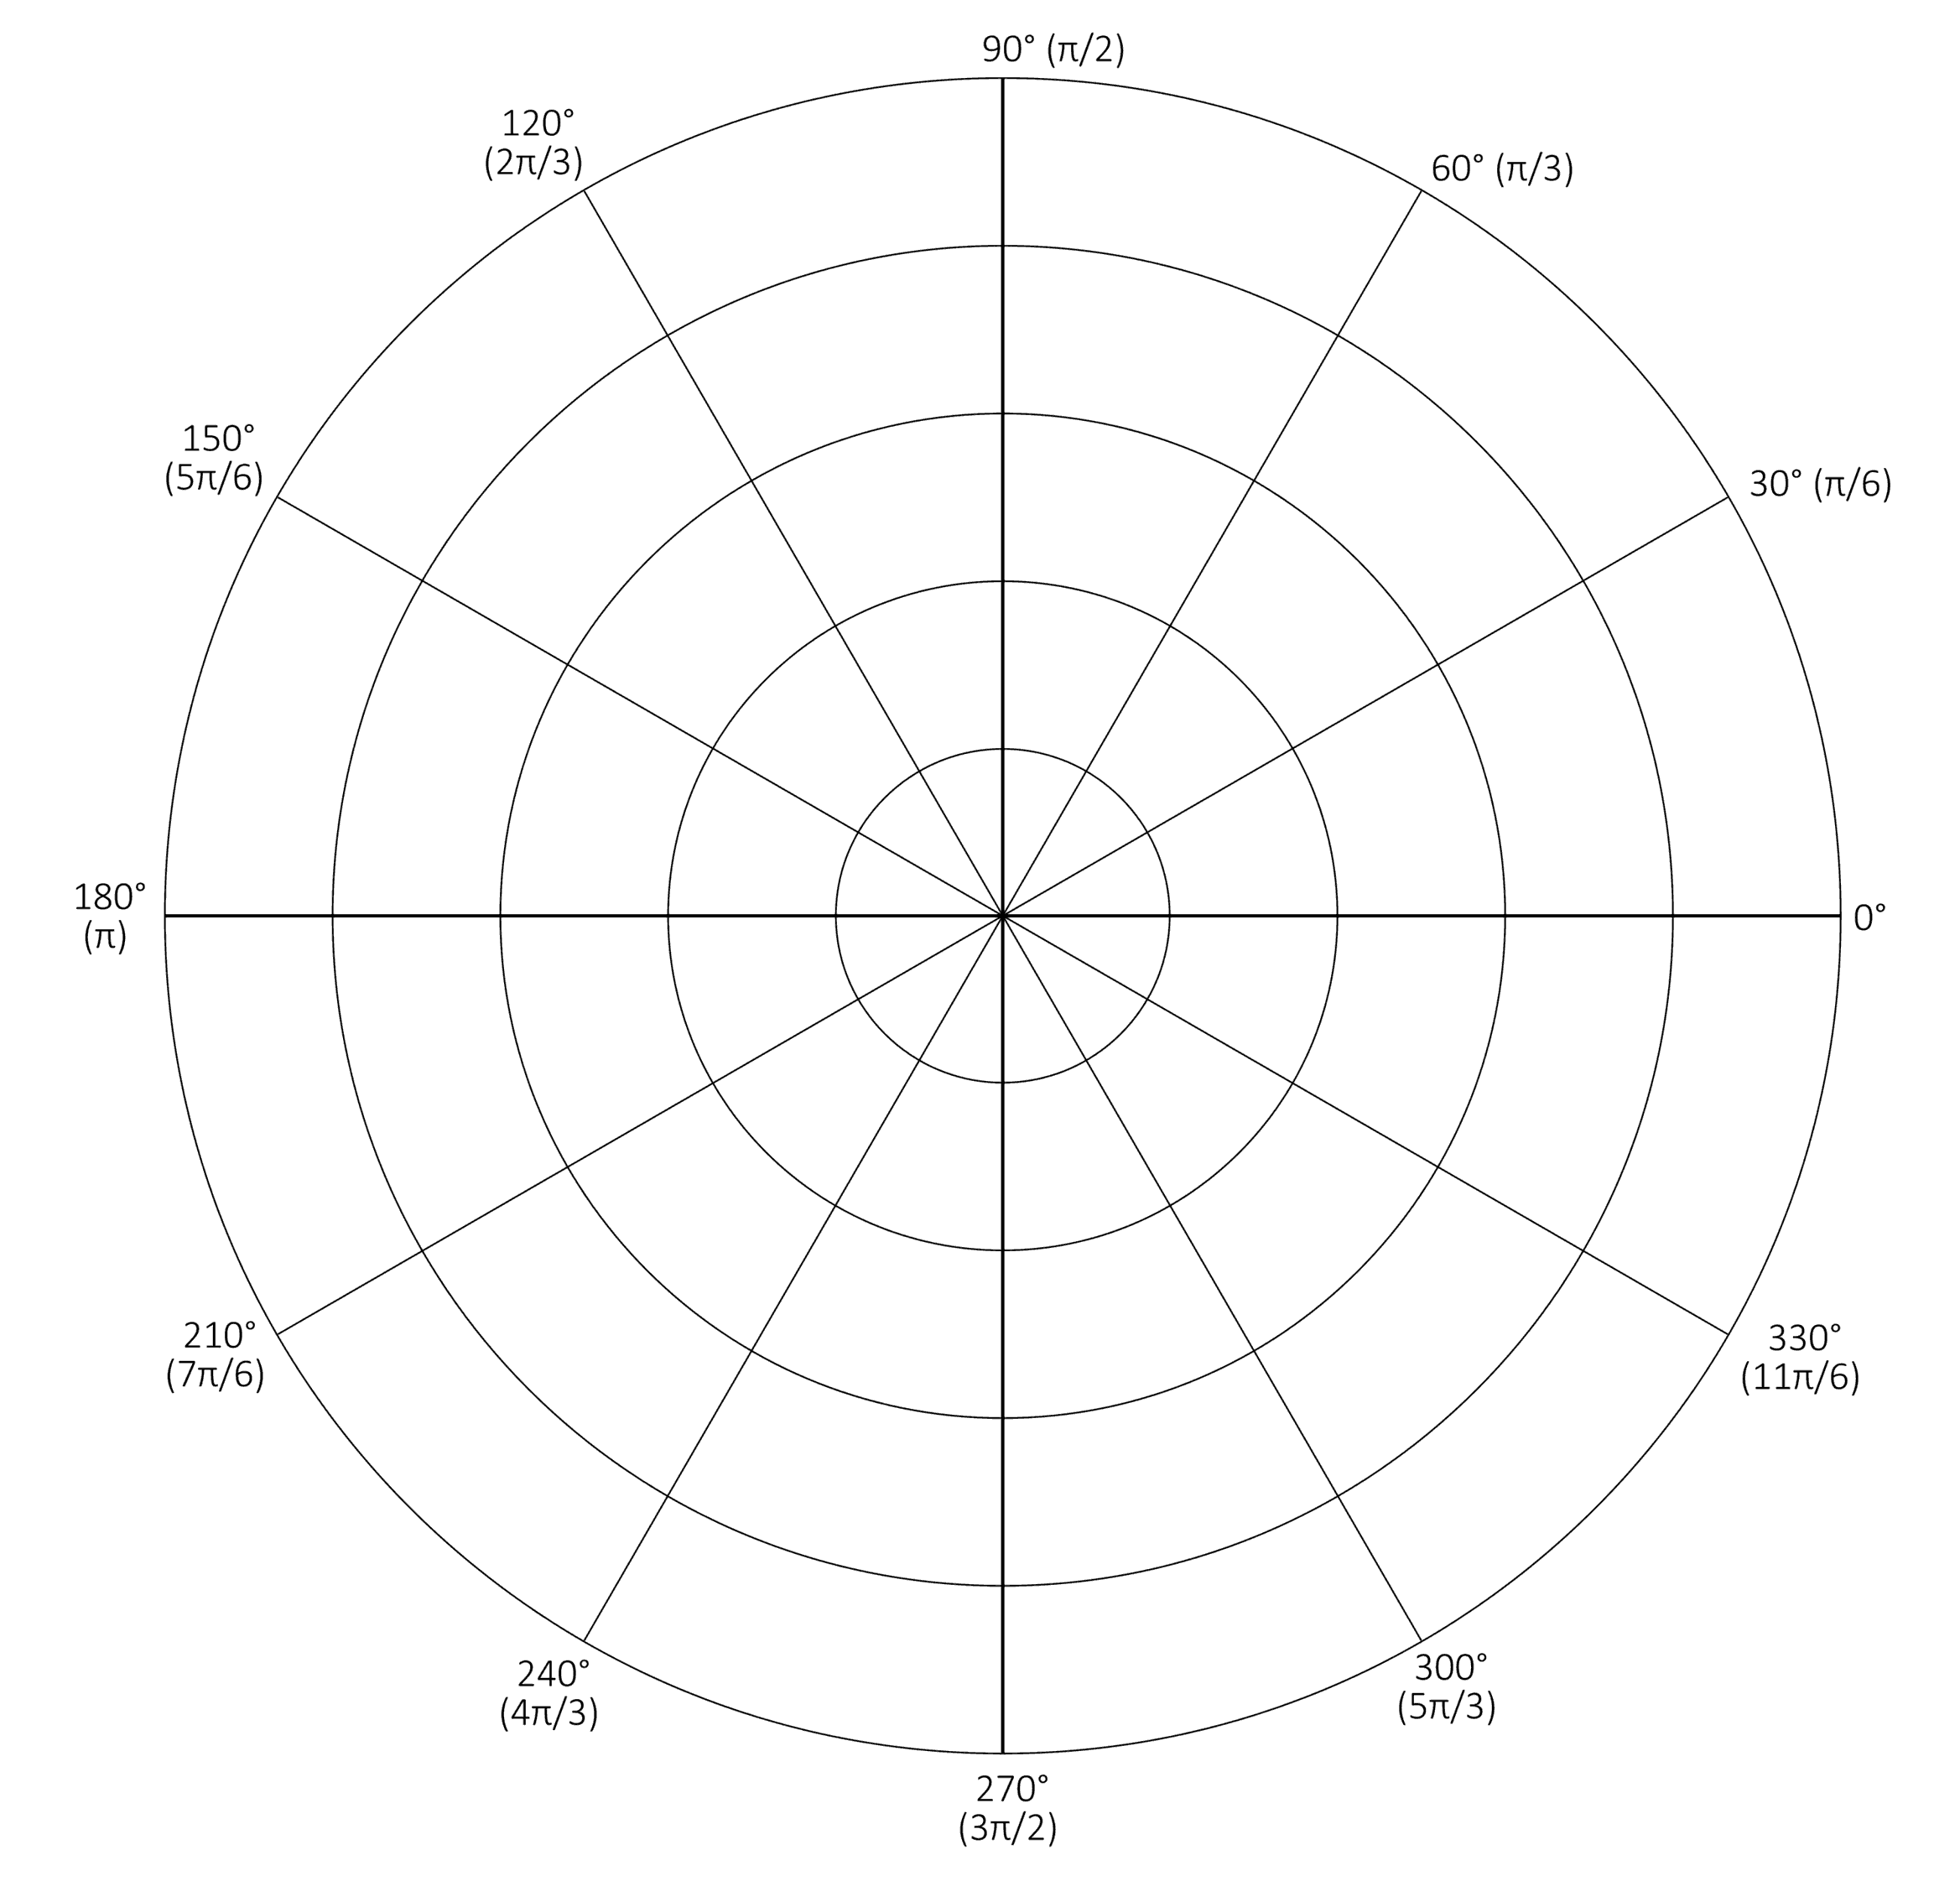
\includegraphics[scale=0.15]{images/polar-graph}
    \end{center}

    \item Does the graph of the curve change if we restrict $\theta$ to only values
    $0 \leq \theta \leq 2\pi$? What about $0 \leq \theta \leq \pi$?
  \end{enumerate}

  
 
  % \begin{center}
  %   \begin{tikzpicture}
  %     \node at (-6,.5){
  %       \begin{tabular}{c|c}
  %         \hline
  %         $\theta$  & $r=1+\sin(\theta)$ \\
  %         \hline
  %         $0$ & $1$ \\
  %         $\pi/6$ & $1+\frac{1}{2} = 1.5$ \\
  %         $\pi/4$ & $1+\frac{\sqrt{2}}{2}\approx 1.7$ \\
  %         $\pi/3$ & $1+\frac{\sqrt{3}}{2}\approx 1.85$ \\
  %         $\pi/2$ & $2$ \\
  %         $-\pi/6$ & $1-\frac{1}{2}=.5$ \\
  %         $-\pi/4$ & $1-\frac{\sqrt{2}}{2}\approx .3$ \\
  %         $-\pi/3$ & $1 - \frac{\sqrt{3}}{2} \approx .15$ \\
  %         $-\pi/2$ & $0$ \\
  %         \hline
  %       \end{tabular}};
  %     % Axis
  %     \draw[->] (-1.5,0) -- (1.5,0) node[right] {$x$}; \draw[->] (0,-1.5) -- (0,2.5) node[above] {$y$};
  %     % Points
  %     \foreach \angle/\radius in { 0/1, 30/1.5, 45/1.7, 60/1.85, 90/2, -30/.5, -45/.3, -60/.15, -90/0} \fill
  %     (\angle:\radius) circle[radius=2pt];
  %   \end{tikzpicture}
  % \end{center}
  % This function has reflection symmetry about the $y$-axis. We can sketch the curve:
  % \begin{center}
  %   \begin{tikzpicture}
  %     % Axis
  %     \draw[->] (-1.5,0) -- (2.5,0) node[right] {$x$};%
  %     \draw[->] (0,-1.5) -- (0,2.5) node[above] {$y$};%
  %     % Curve
  %     \draw[domain=0:360,samples=180,smooth,variable=\t,blue] plot ({\t}:{1 + sin(\t)});%
  %   \end{tikzpicture}
  % \end{center}
\end{problem}



\begin{problem}
  Consider
  \begin{equation*}
    \left\{ \begin{array}{l@{}l} x(t)= 1/t \\ y(t) = 1/t \end{array}\right.
  \end{equation*}
  for $1 \leq t<+\infty$. Sketch the parameterized curve. What is the arc length?
\end{problem}




\end{document}